\documentclass[times,10pt,twocolumn]{article} 
\usepackage{latex8}
\usepackage{times}

\usepackage{amsmath}
\usepackage{times}
\usepackage{comment}
\usepackage{amssymb}
\usepackage{amsmath}
\usepackage{ifthen}
\usepackage{fancyvrb}
\usepackage{multirow}
\usepackage{xspace}
%\usepackage[pdftex]{graphicx}
\usepackage{graphicx}
\usepackage{url}
\usepackage{color} 
\urlstyle{sf}
\usepackage{makeidx}
\usepackage{cite}
\usepackage{url}
\usepackage{rotating}
\usepackage{multirow}
\usepackage{relsize}

%\documentstyle[times,art10,twocolumn,latex8]{article}


\newcommand{\TechReport}[1]{}
\newcommand{\ConfPaper}[1]{#1}
\newboolean{hidecomments}
\setboolean{hidecomments}{false}
\ifthenelse{\boolean{hidecomments}}
{\newcommand{\nb}[2]{}}
{\newcommand{\nb}[2]{
    \fbox{\bfseries\sffamily\scriptsize#1}
    {\sf\small$\blacktriangleright$
      {#2} $\blacktriangleleft$}}}
\newcommand\John[1]{\nb{John}{#1}}
%\newcommand\Danny[1]{\textbf{Danny: {#1}}} 
\newcommand\Danny[1]{\nb{Danny}{#1}}
\newcommand\todo[1]{\fbox{\bfseries\sffamily\scriptsize TODO: #1}}
\newcommand{\tool}{\begin{scriptsize}\textsc{Concurrencer}\end{scriptsize}\xspace}
\newcommand{\toolx}{{\smaller\textsc{Concurrencer}}\xspace}
\newenvironment{CodeOut}{\begin{scriptsize}}{\end{scriptsize}}
\newcommand{\code}[1]{\begin{small}\texttt{#1}\end{small}}
\newcommand{\codex}[1]{{\smaller\texttt{#1}}\xspace}
\newcommand{\myParagraph}[1]{\textbf{#1}}
\newcommand{\HalfWidth}{.40\columnwidth}
\newcommand{\FullWidth}{.95\columnwidth}
\newcommand{\MaxWidth}{\columnwidth}
\newcommand{\ShorterWidth}{.92\columnwidth}
\newcommand{\LongerWidth}{1.08\columnwidth}
\newcommand{\LOCSavedInFJTask}{{302}\xspace}
\newcommand{\humanOmissions}{{41}\xspace}
\newcommand{\LOCchangedTool}{{968}\xspace}
\newcommand{\LOCchangedManually}{{1019}\xspace}
\newcommand{\LOCCouldHaveSavedEditing}{{51}\xspace}
\newcommand{\ConvertToAtomicInteger}{{\begin{scriptsize}\sc{Convert Int to AtomicInteger}\end{scriptsize}}\xspace}
\newcommand{\ConvertToConcurrentHashMap}{{\begin{scriptsize}\sc{Convert HashMap to ConcurrentHashMap}\end{scriptsize}}\xspace}
\newcommand{\ConvertToFJTask}{{\begin{scriptsize}\sc{Convert Recursion to FJTask}\end{scriptsize}}\xspace}
\newcommand{\ConvertToAtomicIntegerx}{{\scriptsize\sc{Convert Int to AtomicInteger}}\xspace}
\newcommand{\ConvertToConcurrentHashMapx}{{\scriptsize\sc{Convert HashMap to ConcurrentHashMap}}\xspace}
\newcommand{\ConvertToFJTaskx}{{\scriptsize\sc{Convert Recursion to FJTask}}\xspace}
%% Define a new 'leo' style for the package that will use a smaller font.
\makeatletter
\def\url@leostyle{%
  \@ifundefined{selectfont}{\def\UrlFont{\sf}}{\def\UrlFont{\small\ttfamily}}}
\makeatother
%% Now actually use the newly defined style.
\urlstyle{leostyle}

%------------------------------------------------------------------------- 
% take the % away on next line to produce the final camera-ready version 
\pagestyle{plain}

%------------------------------------------------------------------------- 
\begin{document}

\title{Concurrencer: a Tool for Retrofitting Concurrency into Sequential Java
Applications via Concurrent Libraries}


\author{Danny Dig, John Marrero, Michael D. Ernst\\
Massachusetts Institute of Technology\\ Computer Science and Artificial
Intelligence Laboratory \\ \{dannydig,marrero,mernst\}@csail.mit.edu\\
}

\maketitle
\thispagestyle{empty}

\begin{abstract}
Parallelizing existing sequential programs to run efficiently on multicores is
hard.  The Java 5 package \code{java.util.concurrent} (\code{j.u.c.}) supports
writing concurrent programs. To use this package, programmers still need to
refactor existing code. This is \emph{tedious}, \emph{error-prone}, and
\emph{omission-prone}.

This demo presents our tool, \tool, which enables programmers to refactor
sequential code into parallel code that uses \code{j.u.c.} concurrent
utilities. \tool does not require any program annotations, although the
transformations span several, non-adjacent, program statements
and use custom program analysis. A find-and-replace tool can not perform
such transformations. Empirical evaluation shows that \tool refactors code
effectively: \tool correctly identifies and applies transformations that some
open-source developers overlooked, and the converted code exhibits good speedup.

\end{abstract}



%------------------------------------------------------------------------- 
\section{Introduction}

% The problem: multicores are here
% For several decades, the computing hardware industry has kept up with Moore's
% Law, effectively doubling the number of transistors per chip every 18 months.
% This translated in roughly doubling the speed of programs that ran
% on the newer machines, an effect dubbed as ``the free performance lunch''.
% Although the hardware industry keeps up with Moore's Law, from now it delivers
% the transistors into multicore chips that run in parallel. This paradigm shift
% demands that programmers find and exploit parallelism in their programs, if they
% want to reap the same performance benefits as in the past.

The computing hardware industry has shifted to multicore processors. This
demands that programmers find and exploit parallelism in their programs, if
they want to reap the same performance benefits as in the past.


% The challenge: parallelize sequential applications
% In the multicore era, a major programming task is to retrofit parallelism into
% the existing sequential programs. It is arguably easier to design 
% the programs with concurrency in mind than to retrofit it
% later~\cite{Lea:CPJ99, Goetz:JCP06}. However, most of the desktop programs were
% not designed to be concurrent, thus programmers have to refactor existing
% sequential programs for concurrency.

% Concrete challenge: thread-safety and scalability
The dominant paradigm for concurrency in desktop programs is shared-memory,
thread-based. However, this paradigm increases the risk for deadlocks and
data-races, commonly known as \emph{thread-safety} concerns. In addition, the
programmer needs to consider \emph{scalability} concerns as well: will the
parallelized program continue to run faster when adding more parallel 
resources? 

% Java.util.concurrent class library
To meet the needs of programmers with respect to thread-safety and scalability,
the Java standard library has been extended with a package,
\code{java.util.concurrent} (from here on referred as \code{j.u.c.}), containing
several utility classes for dealing with concurrency. Among others,
\code{j.u.c.} contains a set of \code{Atomic} classes which offer thread-safe,
lock-free programming over single variables, and several thread-safe abstract
data types (e.g., \code{ConcurrentHashMap}) optimized for scalability. Java 7
will contain a framework \code{Fork/Join
Task}\footnote{http://gee.oswego.edu/dl/concurrency-interest/} for fine-grained
parallelism of intensive computations.


However, manually refactoring a program to use \code{j.u.c.} utilities
is \emph{tedious} because it requires changing many lines
of code, is \emph{error-prone} because programmers can use the wrong APIs,
and is \emph{omission-prone} because programmers can miss opportunities to
use the enhanced APIs.


% This paper presents \tool and three automated refactorings:

This demo presents \tool, our extension to Eclipse's refactoring
engine. \tool enables Java programmers to quickly and safely refactor their sequential
programs to use \code{j.u.c.} utilities. In this demo we present three 
refactorings: (i) \ConvertToAtomicInteger, (ii)
\ConvertToConcurrentHashMap, and (iii) \ConvertToFJTask. 

The first two refactorings are ``enabling transformations'', i.e.,
they make a program thread-safe, but do not introduce multi-threading into a
single-threaded program. Our previous
study~\cite{Dig'08:studyOfConcurrentTransformations} of five open-source
projects that were manually parallelized by their developers shows that these
two refactorings were among some of the most commonly used in practice.
The third refactoring introduces multi-threading: it converts a
sequential recursive divide-and-conquer algorithm into one which solves the
subproblems in parallel using \code{ForkJoinTask}s. 

% Preliminary experience with the refactorings
For evaluation, we compared the manually refactored code in 6
open-source projects with code refactored automatically. The results show
that \tool is effective and the parallel code exhibits good speedup.

A more detailed description of \tool can be found in the ICSE'09
research track~\cite{Dig'09:Concurrencer}.
\tool can be downloaded from:
\code{http://refactoring.info/tools/Concurrencer}

\section{Concurrencer}

\myParagraph{Supported Refactorings.}
% ConvertToAtomicInteger
The first refactoring, \ConvertToAtomicInteger, enables a programmer to
convert an \code{int} field to an \code{AtomicInteger}. \code{AtomicInteger} is
a lock-free utility class which encapsulates an \code{int} value and provides
update operations that execute \emph{atomically}. Our refactoring replaces field
updates with calls to \code{AtomicInteger}'s APIs.

For example, a common update pattern on
an \code{int} field is (i) read the current value, (ii) add delta, and (iii)
update the field value. To make this update thread-safe, the three
operations need to execute \emph{atomically}. Traditionally, programmers use
locks to ensure atomicity. Due to the program having to frequently acquire and
release the lock, the program does not scale well under heavy lock-contention.
\tool finds such read/add/update code patterns and replaces them with a call to
\code{AtomicInteger}'s \code{getAndAdd()} which \emph{atomically} executes the
update without locks (instead it uses efficient compare-and-swap).
 


% ConvertToConcurrentHashMap 
The second refactoring, \ConvertToConcurrentHashMap, enables a programmer
to convert an \code{HashMap} field to \code{ConcurrentHashMap}, a thread-safe,
highly scalable implementation for hash maps. Our refactoring replaces map
update patterns with calls to \code{ConcurrentHashMap}'s atomic APIs. 

For example, a common update pattern is (i) check if a map contains a
$\langle key, value \rangle$ pair, and if it is not present, (ii) place the pair in the map.
For thread-safety, the two operations need to execute atomically. Traditionally,
a programmer would use a map-common lock. Since all accesses to the map have to
acquire the map's lock, this can severely degrade the map's performance.
\tool replaces such an updating pattern with a call to
\code{ConcurrentHashMap}'s \code{putIfAbsent} which \emph{atomically} executes
the update without locking the entire map.

%ConvertToFJTask
The third refactoring, \ConvertToFJTask, converts a sequential
divide-and-conquer algorithm into an algorithm which solves the
recursive subproblems in parallel using the \code{Fork/Join Task} framework. Our
refactoring encapsulates the subproblems as \code{ForkJoinTask}s and passes
them to the framework for effective scheduling.

For example, a sequential \code{mergeSort(array)} first checks
whether the input array is of trivial size (and sorts it directly), otherwise
splits the array into two halves, sorts each half, and then merges
the sorted halves. \tool parallelizes this algorithm using the skeleton of the
sequential algorithm. For the base-case it (i) checks whether the
array is smaller than a user-defined threshold and (ii) invokes the original
sequential sort. For the recursive case, it creates \code{ForkJoinTask}s for
each of the two halves, schedules the two tasks in parallel, waits for the computations to
finish, and then merges the two sorted halves. 

\myParagraph{Implementation.}
% \tool implemented as an Eclipse plugin
\tool is implemented as an extension to Eclipse's refactoring engine, thus it
conveniently provides previewing the code changes, undo, etc. The
programmer only needs select the method or field to be refactored, and the concurrency refactoring (and the sequential threshold
in case of \ConvertToFJTask). 

% enabling program analysis
\tool's program analysis determines (i) whether it
is safe to remove synchronization locks that might protect field accesses, (ii)
its data-flow analysis determines what variables are written in the update
patterns and read afterward, and assigns them appropriately when the
update pattern is replaced with a single API call. The analysis and the code
edits are implemented on top of Eclipse's \code{JDT}.

\myParagraph{Evaluation.}
We used \tool to refactor the same fields that the open-source developers of
Tomcat, MINA, JaxLib, Zimbra, GlassFish, and Struts refactored
to \code{AtomicInteger} or \code{ConcurrentHashMap}. There were a total of 141
such refactorings. Using \tool, the developers could have
saved changing 1019 LOC manually. 

We then compared the manually vs. automatically refactored programs. In terms of
errors in using the {j.u.c.} APIs, the open source developers 4 times
erroneously replaced infix expressions like \code{++f} with
\code{f.getAndIncrement()} (which corresponds to the postfix expression
\code{f++}). \tool used the correct API calls. In terms of missing opportunities
to convert from old update patterns to the new atomic APIs, the programmers
missed 43 out of 83 such opportunities. \tool only missed 10 opportunities.


We also used \tool to parallelize 6 divide-and-conquer algorithms using
\ConvertToFJTask. \tool changed 302 LOC and the parallelized code exhibits on
average 1.84x speedup on a 2-core machine and 3.28x speedup on a 4-core
machine.

\section{Conclusions}
Refactoring sequential code to concurrency is not trivial. Even
seemingly simple refactorings like replacing data types with thread-safe,
scalable implementations provided in \code{java.util.concurrent}, is prone to
human errors and omissions. This demo presents \tool which automates three
refactorings. Our preliminary experience with \tool shows that it
is more effective than a human developer in identifying and applying such
transformations.

%\bibliography{./biblio}
\bibliographystyle{abbrv}
\begin{thebibliography}{10}
\begin{scriptsize}
\bibitem{Dig'08:studyOfConcurrentTransformations}
D.~Dig, J.~Marrero, and M.~D. Ernst.
\newblock How Do Programs Become More Concurrent? {A} Story of Program
  Transformations.
\newblock Tech Report MIT-CSAIL-TR-2008-053.

\bibitem{Dig'09:Concurrencer}
D.~Dig, J.~Marrero, and M.~D. Ernst.
\newblock Refactoring Sequential Java Code for Concurrency via Concurrent
  Libraries.
\newblock To Appear in Proceedings of ICSE'09.
\end{scriptsize}
\end{thebibliography}

%\appendix
%\section{Demo Script}
%
%1. Start with a few slides (2 -3) for motivating the problem of evolving
%existing sequential code to concurrency. \\
%
%
%2. A few slides for presenting the following concurrency features in
%\code{java.util.concurrent} library: \code{Atomics}, \code{ConcurrentHashMap},
%\code{ForkJoinTask}s. \\
%
%
%3. Demonstrate each of the three refactorings by applying the refactoring on
%some real-world code (we have several such real-world codes inspired from the
%6 open-source projects used in the evaluation). \\
%
%
%\emph{Note}: strive to make the demo \emph{interactive} and to engage the
%audience to \emph{ask questions}.
%
%
%
%\section{Screenshots}
%The screenshots are also available in higher resolution at:
%\code{http://refactoring.info/tools/Concurrencer}
%
%\begin{figure*}[htp]
%\begin{center}
%  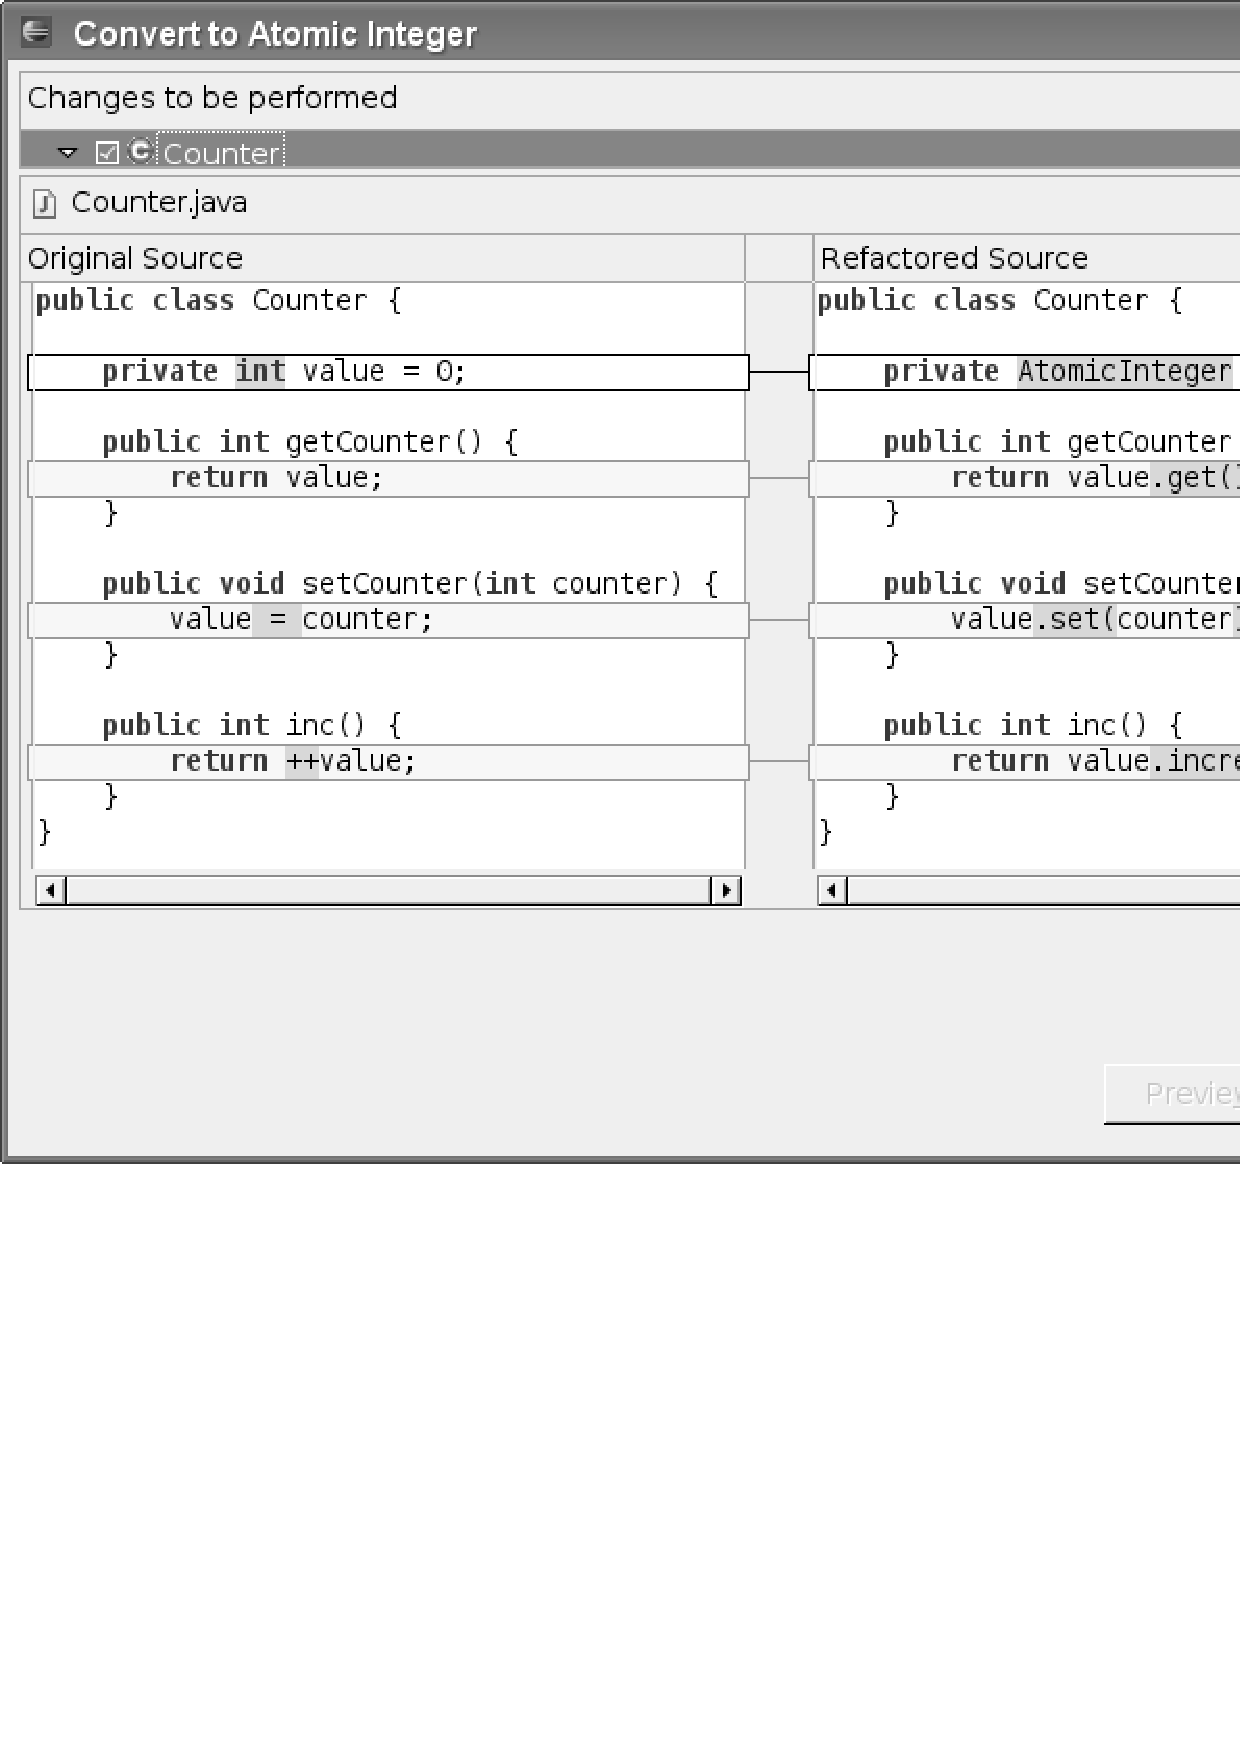
\includegraphics[width=5in]{./figs/ConvertToAtomicInteger.jpg}
%  \caption{Using \toolx to convert an \codex{int} to \codex{AtomicInteger} in Apache Tomcat.
%Left/right shows code before/after refactoring.}
%  \label{fig:CounterExample}
%\end{center}
%%\vspace{-0.4 in}
%\end{figure*}
%
%
%\begin{figure*}[htp]
%\begin{center}
%  \includegraphics[width=5.5in]{./figs/ConvertToConcurrentHashMap.jpg}
%  \caption{Using \toolx to convert an \codex{HashMap} field to
%  \codex{ConcurrentHashMap}. Left/right shows code before/after
%  refactoring.}
%  \label{fig:ConvertToCHM}
%\end{center}
%%\vspace{-0.4 in}
%\end{figure*}
%
%\begin{figure*}[htp]
%\begin{center}
%  \includegraphics[width=7.5in]{./figs/ConvertSortToFJTask.JPG}
%  \caption{\toolx converts a sequential divide-and-conquer \codex{mergeSort} algorithm into an algorithm that solves
%  the subproblems in parallel using Java 7's \codex{ForkJoinTask} framework. Left/right shows code before/after
%  refactoring. The programmer needs only provide the sequential threshold condition, \codex{whole.length < 100}}
%  \label{fig:ConvertToFJTask}
%\end{center}
%%\vspace{-0.4 in}
%\end{figure*}

\end{document}